\documentclass{article}

% import packages
\usepackage{amsmath,amsfonts,amsthm,amssymb,amsopn,bm}
\usepackage{mathtools}
\usepackage[margin=.9in]{geometry}
\usepackage{graphicx}
\usepackage[dvipsnames]{xcolor}
\usepackage{minted}
\usepackage{subcaption}
\usepackage{float}
\usepackage{multicol}

% note command
\newcommand{\note}[1]{\textsf{\textcolor{Red}{#1}}}

% some math commands
\newcommand{\norm}[1]{\left\|#1\right\|}
\newcommand{\twonorm}[1]{\|#1\|_2^2}
\newcommand{\vect}[1]{\boldsymbol{#1}} % vector 
\DeclareMathOperator{\E}{\mathbb{E}}
\DeclareMathOperator{\R}{\mathbb{R}}
\DeclareMathOperator{\cov}{Cov}
\DeclareMathOperator{\var}{Var}

% remove indents
\setlength\parindent{0px}
% enumerate with lowercase letters
\renewcommand{\theenumi}{\alph{enumi}}
% indented environment for solutions
\usepackage{changepage}
\newenvironment{solution}{\begin{adjustwidth}{8mm}{}}{\end{adjustwidth}}

\setlength{\columnsep}{-4cm}

% Homework title and date
\renewcommand{\title}{Homework 4}
\renewcommand{\date}{December 16, 2020}

\begin{document}

\begin{center}
        \LARGE \title \\ \vspace{10pt}
        \normalsize 
        Fall 2020, CSE 546: Machine Learning \\ \vspace{2pt}
        John Franklin Crenshaw \\ \vspace{2pt}
        \date
\end{center}

%Collaborators:

\section*{Section 1}

A.1

\begin{enumerate}
    \item True. This can be problematic as the solution you arrive at can depend on how you initialize your weights.
    \item False. If all of your weights start the same, then the neural network can't ``tell them apart'', and gradient descent will update them all identically.
    This prevents the network from learning.
    \item True. Without these non-linear layers, a neural network would still just be a linear model.
    \item False. In a standard neural network, the backwards pass has the same time complexity as the forward pass.
    \item True. PCA is a linear model, and autoencoders with nonlinear activations are able to learn nonlinear structure, so they are able to capture more variance of the data.
\end{enumerate}

\newpage

A.2
\begin{enumerate}
        \item
        \begin{multicols}{2}
                $h$=32, ~\,training error = 0.022 \\
                $h$=64, ~\,training error = 0.012 \\
                $h$=128, training error = 0.006 \\
                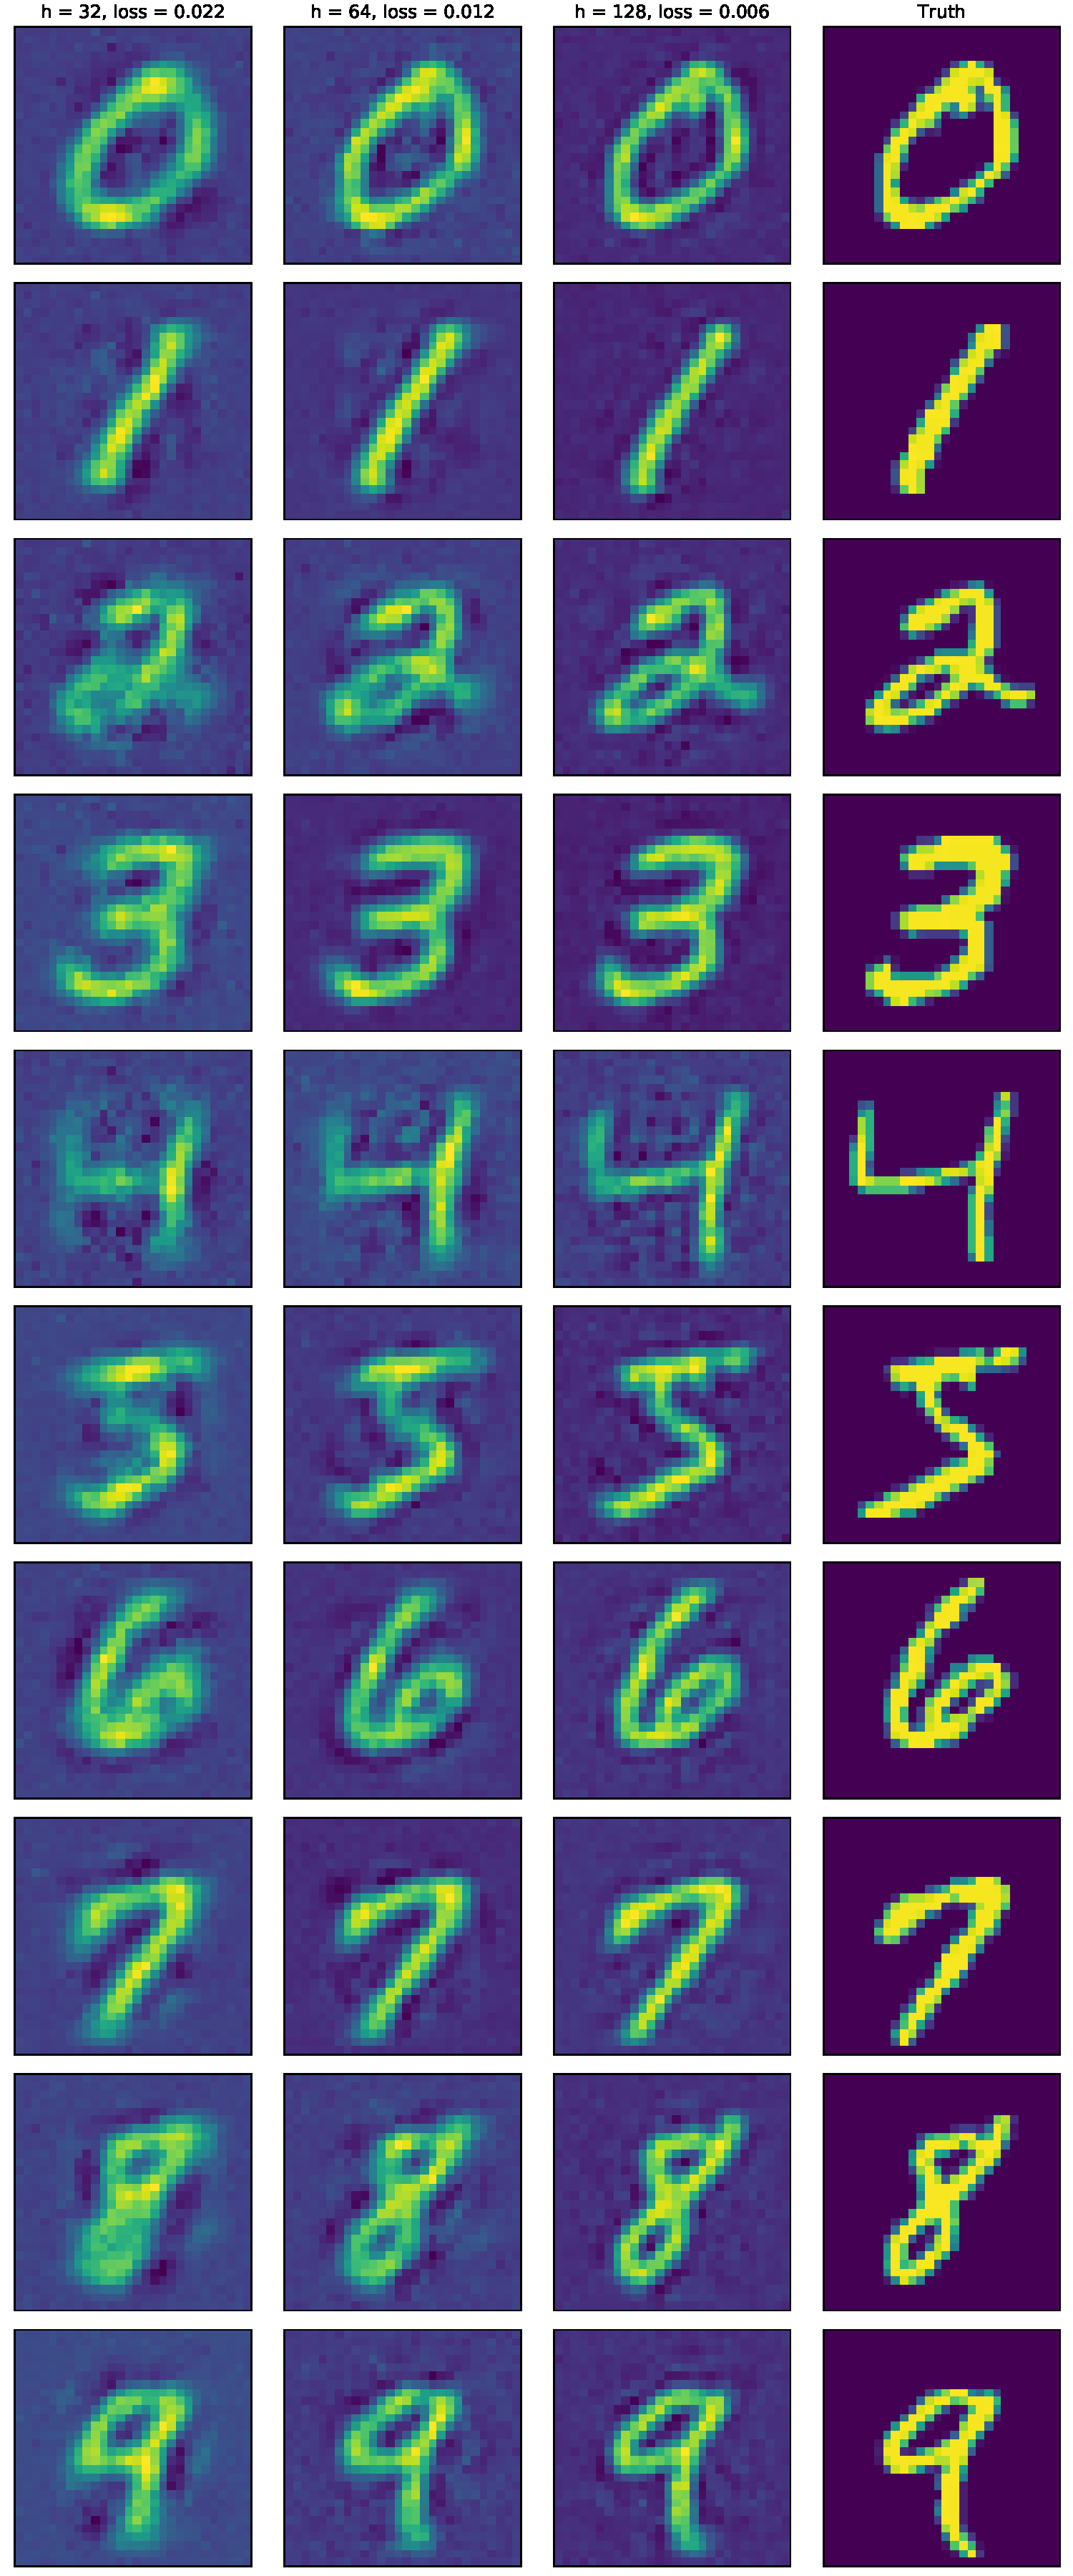
\includegraphics[width=0.55\textwidth]{code/A2a.pdf}
        \end{multicols}
        \begin{minted}{python}
import numpy as np
import matplotlib.pyplot as plt
import torch
from torch.nn import Sequential, Linear, ReLU, MSELoss
from torch.optim import Adam

from mnist import MNIST
def load_dataset():
    mndata = MNIST('../../../python-mnist/data/')
    X_train, labels_train = map(np.array, mndata.load_training())
    X_test, labels_test = map(np.array, mndata.load_testing())
    X_train = X_train/255.0
    X_test = X_test/255.0
    
    return X_train, labels_train, X_test, labels_test

X_train, Y_train, X_test, Y_test = load_dataset()

X_train = torch.from_numpy(X_train).float()
X_test = torch.from_numpy(X_test).float()

# define the autoencoder
def Autoencoder(d, h):
    model = Sequential(
                Linear(d, h),
                Linear(h, d)
            )
    return model

# dimensions for the autoencoder
d = X_train[0].numel()
hs = [32, 64, 128]

# create loss function
mseLoss = MSELoss()

# dictionary to save losses and predictions
save_dict = {h: dict() for h in hs}

# indices for each digit
# will use these to save predictions for each digit
idx = [np.where(Y_train == digit)[0][0] for digit in range(10)]

# loop over values of h
for h in hs:

    # initialize the model
    model = Autoencoder(d, h)

    # create an optimizer
    lr = 1e-3
    optimizer = Adam(model.parameters(), lr=lr)

    # container to save losses throughout training
    losses = []

    # train the model
    for t in range(500):

        # forward pass
        X_pred = model(X_train)

        # calculate loss
        loss = mseLoss(X_pred, X_train)
        losses.append(loss.item())
        if t % 100 == 99:
            print(h, t, loss.item())
            
        # zero out the gradient buffers
        optimizer.zero_grad()

        # backward pass
        loss.backward()

        # use gradient to step parameters
        optimizer.step()
        
    # save save the losses and the predictions
    save_dict[h]['loss'] = losses
    save_dict[h]['X_pred'] = model(X_train[idx]).detach().numpy()

    fig,axes = plt.subplots(10,4, figsize=(10,24), constrained_layout=True)

for j,h in enumerate(save_dict):
    loss = save_dict[h]['loss'][-1]
    axes[0,j].set_title(f'h = {h}, loss = {loss:.3f}')
    X_pred = save_dict[h]['X_pred']
    for i,X in enumerate(X_pred):
        axes[i,j].imshow(X.reshape(28,28))
        axes[i,j].set(xticks=[],yticks=[])

axes[0,-1].set_title('Truth')
X_truth = X_train[idx]
for i,X in enumerate(X_truth):
    axes[i,-1].imshow(X.reshape(28,28))
    axes[i,-1].set(xticks=[],yticks=[])
        \end{minted}
        \newpage

        \item \, \\
        \begin{multicols}{2}
                $h$=32, ~\,training error = 0.021 \\
                $h$=64, ~\,training error = 0.011 \\
                $h$=128, training error = 0.007 \\
                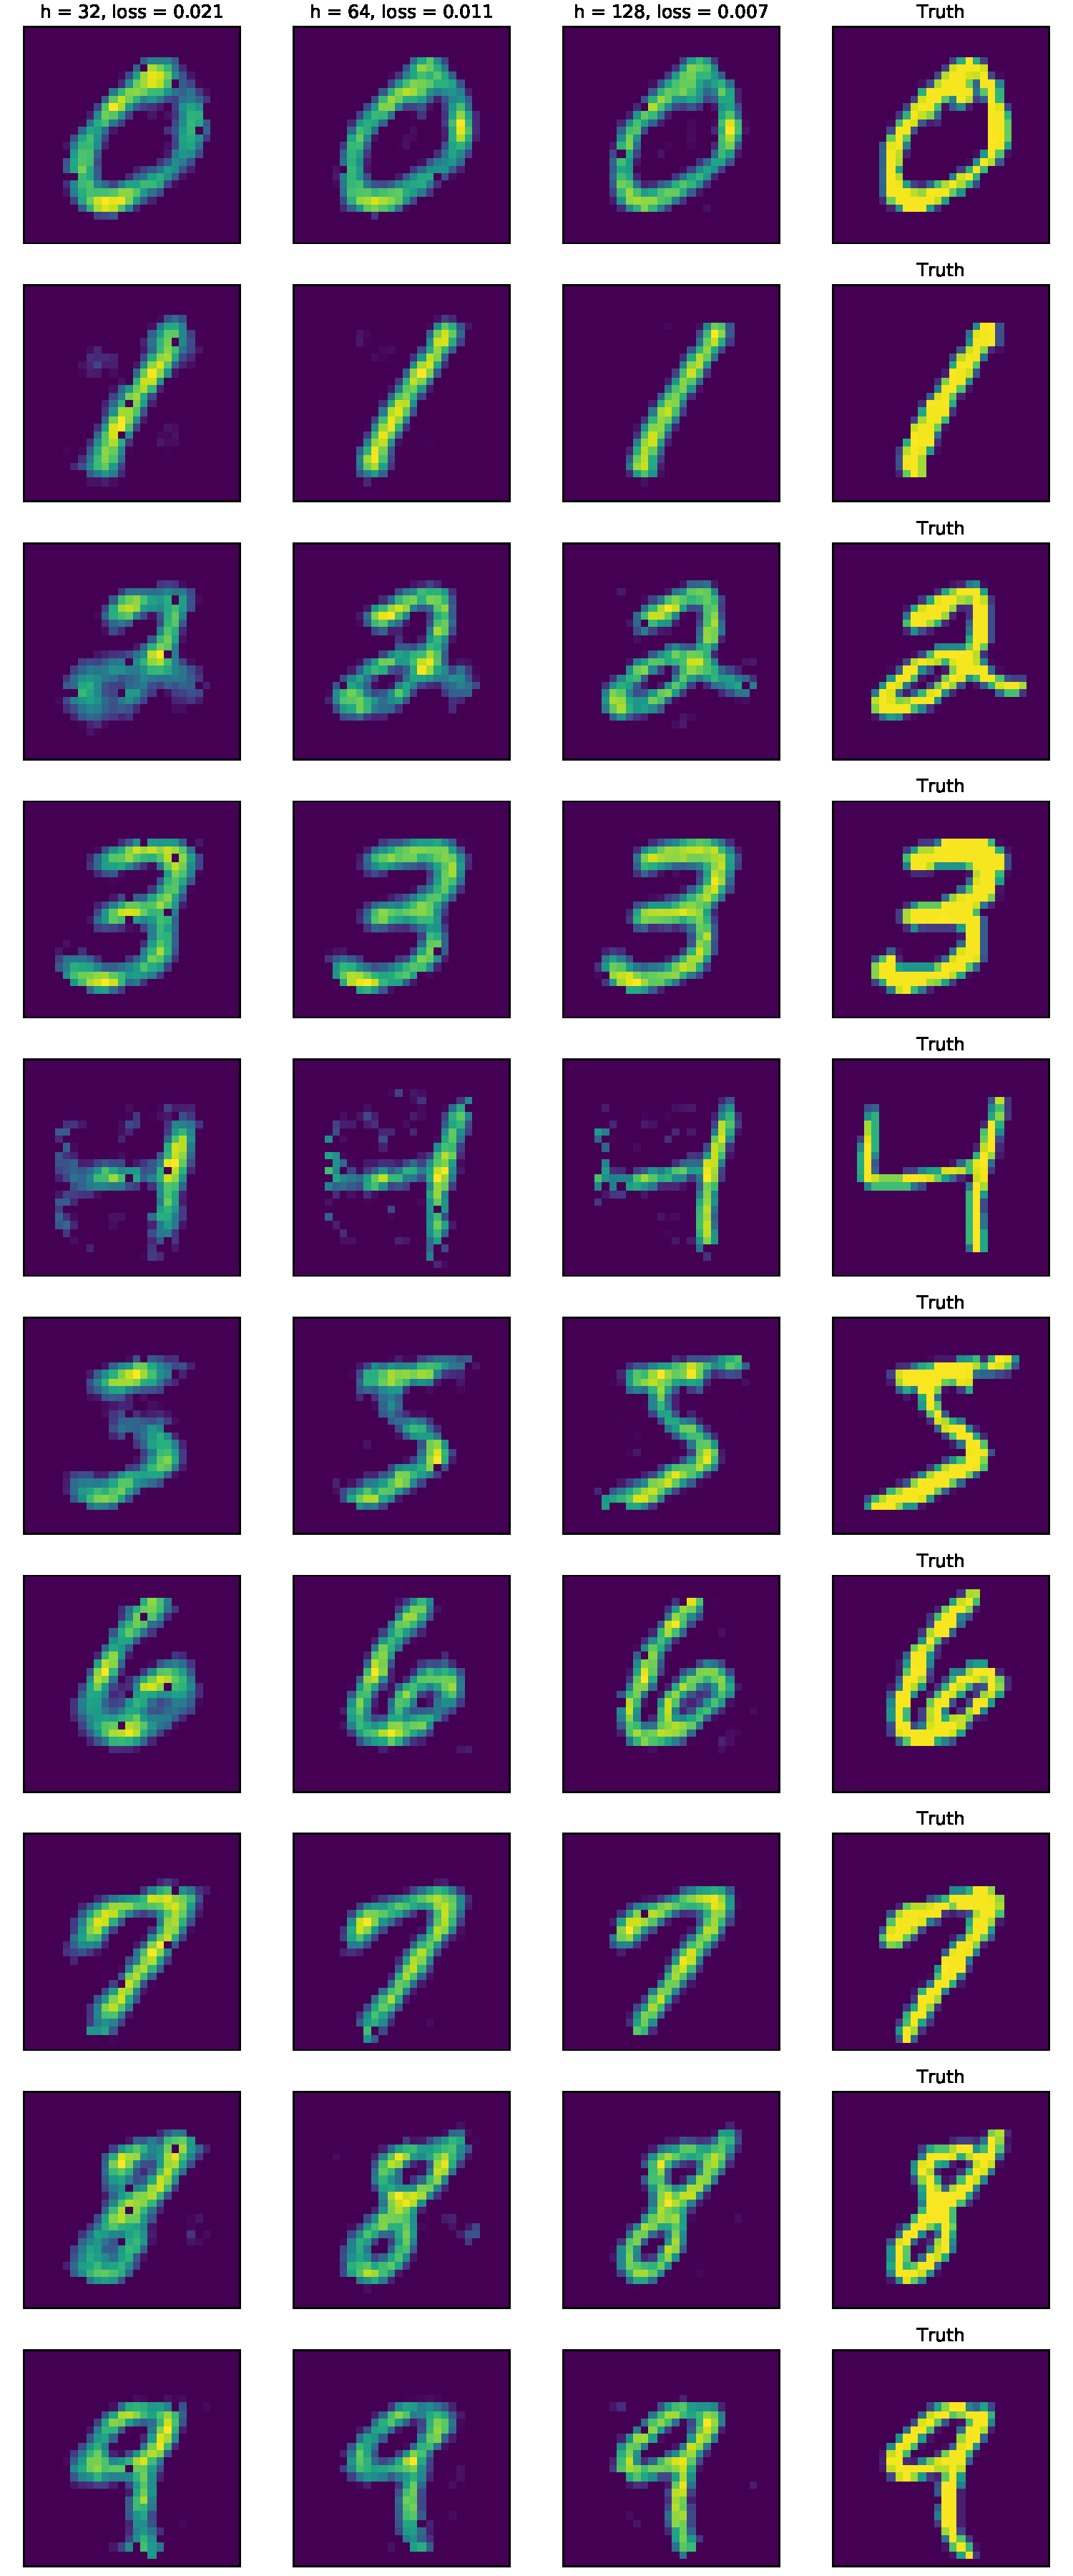
\includegraphics[width=0.55\textwidth]{code/A2b.pdf}
        \end{multicols}
        \begin{minted}{python}
# define the autoencoder
def Autoencoder(d, h):
    model = Sequential(
                Linear(d, h),
                ReLU(),
                Linear(h, d),
                ReLU()
            )
    return model

# dimensions for the autoencoder
d = X_train[0].numel()
hs = [32, 64, 128]

# create loss function
mseLoss = MSELoss()

# dictionary to save losses and predictions
save_dict2 = {h: dict() for h in hs}

# indices for each digit
# will use these to save predictions for each digit
idx = [np.where(Y_train == digit)[0][0] for digit in range(10)]

# loop over values of h
for h in hs:

    # initialize the model
    model2 = Autoencoder(d, h)

    # create an optimizer
    lr = 1e-3
    optimizer = Adam(model2.parameters(), lr=lr)

    # container to save losses throughout training
    losses = []

    # train the model
    for t in range(500):

        # forward pass
        X_pred = model2(X_train)

        # calculate loss
        loss = mseLoss(X_pred, X_train)
        losses.append(loss.item())
        if t % 100 == 99:
            print(h, t, loss.item())
            
        # zero out the gradient buffers
        optimizer.zero_grad()

        # backward pass
        loss.backward()

        # use gradient to step parameters
        optimizer.step()
        
    # save save the losses and the predictions
    save_dict2[h]['loss'] = losses
    save_dict2[h]['X_pred'] = model2(X_train[idx]).detach().numpy()

    fig,axes = plt.subplots(10,4, figsize=(10,24), constrained_layout=True)

for j,h in enumerate(save_dict2):
    loss = save_dict2[h]['loss'][-1]
    axes[0,j].set_title(f'h = {h}, loss = {loss:.3f}')
    X_pred = save_dict2[h]['X_pred']
    for i,X in enumerate(X_pred):
        axes[i,j].imshow(X.reshape(28,28))
        axes[i,j].set(xticks=[],yticks=[])
        
X_truth = X_train[idx]
for i,X in enumerate(X_truth):
    axes[i,-1].set_title('Truth')
    axes[i,-1].imshow(X.reshape(28,28))
    axes[i,-1].set(xticks=[],yticks=[])
        \end{minted}

        \item
        $\mathcal{F}_1$ recon err 0.0061 \\
        $\mathcal{F}_2$ recon err 0.0066
        
        \item The autoencoder reconstructions are much better than the PCA reconstructions, and in particular are much sharper.
        This makes sense as sharp boundaries are typically non-linear features.
        Here are the PCA reconstructions where you can see that the images are fuzzier. \\
        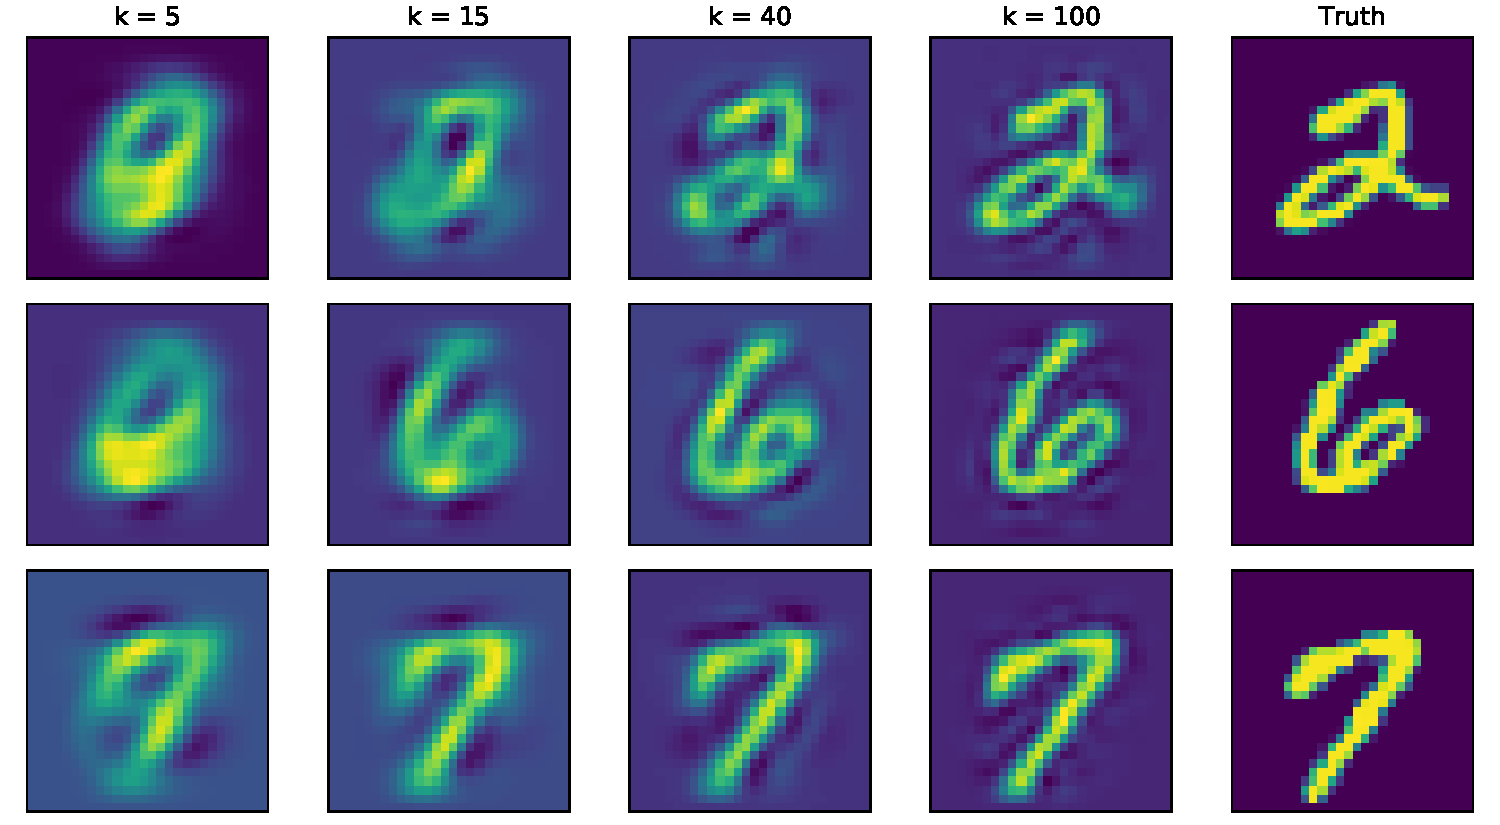
\includegraphics[width=0.8\textwidth]{../hw3/code/A7e.pdf}
\end{enumerate}

\newpage

A.3
\begin{enumerate}
        \item \, \\
        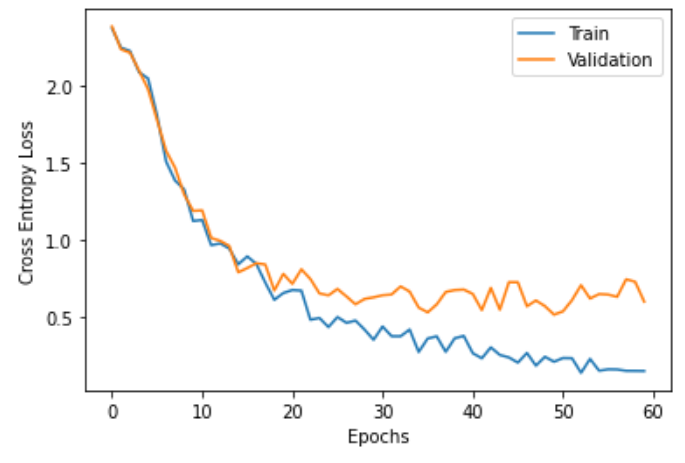
\includegraphics[width=0.6\textwidth]{code/A3a.png} \\
        Highest validation accuracy: 0.83 \\
        Test accuracy: 0.83 \\
        Test loss: 0.577
        \begin{minted}{python}
import numpy as np
import matplotlib.pyplot as plt
import torch

# alexnet
from torchvision.models import alexnet
from torch.nn import Linear

# cifar10
from torchvision.datasets import CIFAR10
import torchvision.transforms as transforms
from torch.utils.data import DataLoader

# optimizer and loss
from torch.optim import Adam
from torch.nn import CrossEntropyLoss

device = torch.device('cuda:0' if torch.cuda.is_available() else 'cpu')

model = alexnet(pretrained=True)
for param in model.parameters():
    param.required_grad = False
model.classifier[6] = Linear(4096, 10)
model.to(device);

transform = transforms.Compose([transforms.Resize((256, 256)), transforms.ToTensor()])

trainset = CIFAR10(root='.', train=True, download=True, transform=transform)
trainloader = DataLoader(trainset, batch_size=512, shuffle=True, num_workers=2)

testset = CIFAR10(root='.', train=False, download=True, transform=transform)
testloader = DataLoader(testset, batch_size=512, shuffle=True, num_workers=2)

optimizer = Adam(model.parameters(), lr=1e-3)
loss_fn = CrossEntropyLoss()

trainlosses = []
testlosses = []

for i in range(60):
  print(i)
  for j, data in enumerate(zip(trainloader,testloader)):
    # unpack data
    trainI, trainL = data[0][0].to(device), data[0][1].to(device)
    testI, testL = data[1][0].to(device), data[1][1].to(device)

    # validation loss
    output = model(testI)
    testloss = loss_fn(output, testL)
    testlosses.append(testloss.item())

    # train loss
    output = model(trainI)
    trainloss = loss_fn(output, trainL)
    trainlosses.append(trainloss.item())

    # backprop
    optimizer.zero_grad()
    trainloss.backward()
    optimizer.step()

    if j % 5 == 4:
      print(trainloss.item())

plt.plot(trainlosses[::20], label='Train')
plt.plot(testlosses[::20], label='Validation')
plt.xlabel('Epochs')
plt.ylabel('Cross Entropy Loss')
plt.legend()
plt.show()

output = model(testI)
predLabel = output.cpu().detach().numpy().argmax(axis=1)
trueLabel = testL.cpu().detach().numpy()
len(predLabel[predLabel == trueLabel])/len(predLabel)
        \end{minted} 
        
        \newpage

        \item \, \\
        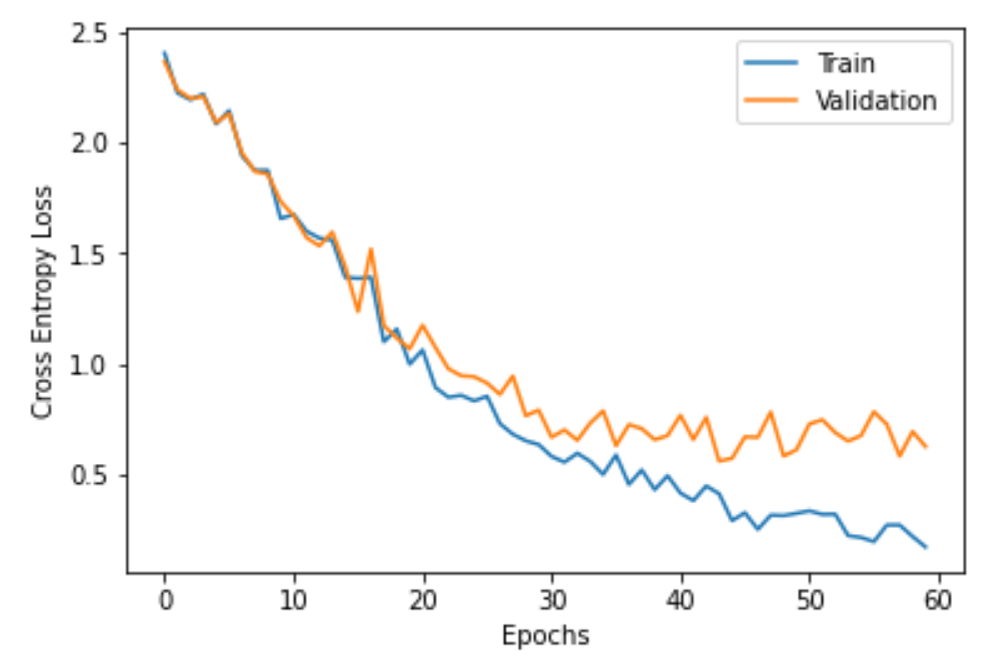
\includegraphics[width=0.6\textwidth]{code/A3b.png} \\
        Highest validation accuracy: 0.79 \\
        Test accuracy: 0.79 \\
        Test loss: 0.556 \\
        The code is identical to that above, except \textit{without} the lines
        \begin{minted}{python}
for param in model.parameters():
    param.required_grad = False
        \end{minted}
\end{enumerate}

\newpage

A.4

\begin{enumerate}
        \item I tried a search of learning rate, with values of 0.01, 0.001, 0.0001.
        The best result was with a learning rate of 0.001.
        Below are the training and validation accuracies for each hyperparameter set.
        The train accuracies are solid and the validation accuracies are dashed. \\
        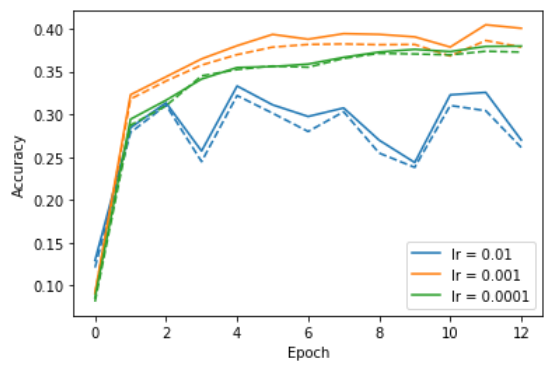
\includegraphics[width=0.7\textwidth]{code/A4a.png} \\
        The test accuracy for the best hyperparameters is 0.374
        \begin{minted}{python}
import torch
import torchvision
import torchvision.transforms as transforms
from torch.utils.data import random_split
device = torch.device("cuda:0" if torch.cuda.is_available() else "cpu")

import matplotlib.pyplot as plt

transform = transforms.Compose([transforms.ToTensor()])

trainset = torchvision.datasets.CIFAR10(root='./data', train=True,
                                        download=True, transform=transform)
valset, trainset = random_split(trainset, [10000, 40000])
trainloader = torch.utils.data.DataLoader(trainset, batch_size=512,
                                          shuffle=True, num_workers=1)

testset = torchvision.datasets.CIFAR10(root='./data', train=False,
                                       download=True, transform=transform)
testloader = torch.utils.data.DataLoader(testset, batch_size=len(testset),
                                         shuffle=False, num_workers=1)

classes = ('plane', 'car', 'bird', 'cat',
           'deer', 'dog', 'frog', 'horse', 'ship', 'truck')

           import torch.nn as nn
import torch.nn.functional as F


class Net(nn.Module):
    def __init__(self):
        super(Net, self).__init__()
        self.fc1 = nn.Linear(3072, 10)

    def forward(self, x):
        x = x.reshape(-1, 3072)
        x = self.fc1(x)
        return x

        import torch.optim as optim

criterion = nn.CrossEntropyLoss()

results = {1: {'hyperparams': {'lr': 0.01},
               'train_acc': [], 'val_acc': []},
           2: {'hyperparams': {'lr': 0.001},
               'train_acc': [], 'val_acc': []},
           3: {'hyperparams': {'lr': 0.0001},
               'train_acc': [], 'val_acc': []}}

               for V in results.values():

print(V['hyperparams'])

net = Net()
net.to(device)

optimizer = optim.Adam(net.parameters(), lr=V['hyperparams']['lr'])

for epoch in range(13):  # loop over the dataset multiple times

    if epoch > 0:
      for i, data in enumerate(trainloader):
          # get the inputs; data is a list of [inputs, labels]
          inputs, labels = data[0].to(device), data[1].to(device)
          
          # zero the parameter gradients
          optimizer.zero_grad()

          # forward + backward + optimize
          outputs = net(inputs)
          loss = criterion(outputs, labels)
          loss.backward()
          optimizer.step()

    inputs = torch.tensor(trainset.dataset.data[trainset.indices].transpose(0,3,1,2)).float().to(device)
    labels = torch.tensor(trainset.dataset.targets)[trainset.indices].float().to(device)
    outputs = net(inputs).argmax(axis=1)
    train_acc = len(outputs[outputs==labels])/len(outputs)
    V['train_acc'].append(train_acc)

    inputs = torch.tensor(valset.dataset.data[valset.indices].transpose(0,3,1,2)).float().to(device)
    labels = torch.tensor(valset.dataset.targets)[valset.indices].float().to(device)
    outputs = net(inputs).argmax(axis=1)
    val_acc = len(outputs[outputs==labels])/len(outputs)
    V['val_acc'].append(val_acc)

    print(f'Epoch: {epoch:>2}    Train Acc: {train_acc:.3f}    Val Acc: {val_acc:.3f}')

print('Finished Training')

inputs = torch.tensor(testset.data.transpose(0,3,1,2)).float().to(device)
labels = torch.tensor(testset.targets).float().to(device)
outputs = net(inputs).argmax(axis=1)
test_acc = len(outputs[outputs==labels])/len(outputs)
print(f"Test Acc {test_acc:.3f}")

for i,V in enumerate(results.values()):
  plt.plot(V['train_acc'], c=f'C{i}', label=f"lr = {V['hyperparams']['lr']}")
  plt.plot(V['val_acc'], c=f'C{i}', ls='--')

plt.xlabel('Epoch')
plt.ylabel('Accuracy')

plt.legend()
plt.show()
        \end{minted}

        \newpage
        \item I fixed the learning rate at 0.001, and searched $M$ in intervals of 20 over the range 100 to 240.
        The best result was with $M = 200$.
        Below are the training and validation accuracies for each hyperparameter set.
        The train accuracies are solid and the validation accuracies are dashed. \\
        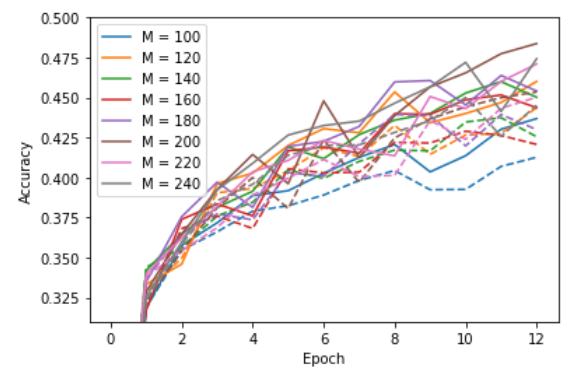
\includegraphics[width=0.7\textwidth]{code/A4b.png} \\
        The test accuracy for the best hyperparameters is 0.456.
        \begin{minted}{python}
import torch
import torchvision
import torchvision.transforms as transforms
from torch.utils.data import random_split
device = torch.device("cuda:0" if torch.cuda.is_available() else "cpu")

import matplotlib.pyplot as plt

transform = transforms.Compose([transforms.ToTensor()])

trainset = torchvision.datasets.CIFAR10(root='./data', train=True,
                                        download=True, transform=transform)
valset, trainset = random_split(trainset, [10000, 40000])
trainloader = torch.utils.data.DataLoader(trainset, batch_size=512,
                                                shuffle=True, num_workers=1)

testset = torchvision.datasets.CIFAR10(root='./data', train=False,
                                        download=True, transform=transform)
testloader = torch.utils.data.DataLoader(testset, batch_size=len(testset),
                                                shuffle=False, num_workers=1)

classes = ('plane', 'car', 'bird', 'cat',
                'deer', 'dog', 'frog', 'horse', 'ship', 'truck')

import torch.nn as nn
import torch.nn.functional as F


class Net(nn.Module):
        def __init__(self):
        super(Net, self).__init__()
        self.fc1 = nn.Linear(3072, 10)

        def forward(self, x):
        x = x.reshape(-1, 3072)
        x = self.fc1(x)
        return x

import torch.optim as optim

criterion = nn.CrossEntropyLoss()

results = {1: {'hyperparams': {'M': 100},
               'train_acc': [], 'val_acc': []},
           2: {'hyperparams': {'M': 120},
               'train_acc': [], 'val_acc': []},
           3: {'hyperparams': {'M': 140},
               'train_acc': [], 'val_acc': []},
           4: {'hyperparams': {'M': 160},
               'train_acc': [], 'val_acc': []},
           5: {'hyperparams': {'M': 180},
               'train_acc': [], 'val_acc': []},
           6: {'hyperparams': {'M': 200},
               'train_acc': [], 'val_acc': []},
           7: {'hyperparams': {'M': 220},
               'train_acc': [], 'val_acc': []},
           8: {'hyperparams': {'M': 240},
               'train_acc': [], 'val_acc': []}}

for V in results.values():

        print(V['hyperparams'])
        
        net = Net()
        net.to(device)
        
        optimizer = optim.Adam(net.parameters(), lr=V['hyperparams']['lr'])
        
        for epoch in range(13):  # loop over the dataset multiple times
        
                if epoch > 0:
                        for i, data in enumerate(trainloader):
                                # get the inputs; data is a list of [inputs, labels]
                                inputs, labels = data[0].to(device), data[1].to(device)
                                
                                # zero the parameter gradients
                                optimizer.zero_grad()
                        
                                # forward + backward + optimize
                                outputs = net(inputs)
                                loss = criterion(outputs, labels)
                                loss.backward()
                                optimizer.step()
        
                inputs = torch.tensor(trainset.dataset.data[trainset.indices].transpose(0,3,1,2)).float().to(device)
                labels = torch.tensor(trainset.dataset.targets)[trainset.indices].float().to(device)
                outputs = net(inputs).argmax(axis=1)
                train_acc = len(outputs[outputs==labels])/len(outputs)
                V['train_acc'].append(train_acc)
                
                inputs = torch.tensor(valset.dataset.data[valset.indices].transpose(0,3,1,2)).float().to(device)
                labels = torch.tensor(valset.dataset.targets)[valset.indices].float().to(device)
                outputs = net(inputs).argmax(axis=1)
                val_acc = len(outputs[outputs==labels])/len(outputs)
                V['val_acc'].append(val_acc)
        
                print(f'Epoch: {epoch:>2}    Train Acc: {train_acc:.3f}    Val Acc: {val_acc:.3f}')

print('Finished Training')

inputs = torch.tensor(testset.data.transpose(0,3,1,2)).float().to(device)
labels = torch.tensor(testset.targets).float().to(device)
outputs = net(inputs).argmax(axis=1)
test_acc = len(outputs[outputs==labels])/len(outputs)
print(f"Test Acc {test_acc:.3f}")

for i,V in enumerate(results.values()):
        plt.plot(V['train_acc'], c=f'C{i}', label=f"lr = {V['hyperparams']['lr']}")
        plt.plot(V['val_acc'], c=f'C{i}', ls='--')

plt.xlabel('Epoch')
plt.ylabel('Accuracy')

plt.legend()
plt.show()
                        \end{minted}

        \newpage
        \item I increased the number of filters to 200 and decreased the max pooling size to 8, but, per the instructions, did not perform a full hyperparameter search.
        These values reached the desired training accuracy. 
        The final test accuracy was 65\%. \\
        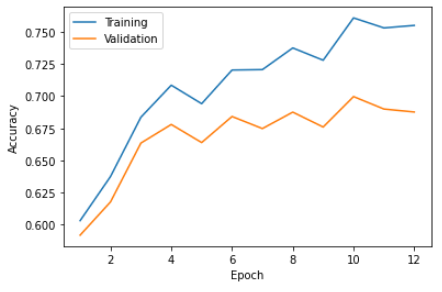
\includegraphics[width=0.5\textwidth]{code/A4c.png}
        \begin{minted}{python}
import torch
import torchvision
import torchvision.transforms as transforms
from torch.utils.data import random_split
device = torch.device("cuda:0" if torch.cuda.is_available() else "cpu")

transform = transforms.Compose(
    [transforms.ToTensor(),
     transforms.Normalize((0.5, 0.5, 0.5), (0.5, 0.5, 0.5))])

trainset = torchvision.datasets.CIFAR10(root='./data', train=True,
                                        download=True, transform=transform)
valset, trainset = random_split(trainset, [10000,40000])
trainloader = torch.utils.data.DataLoader(trainset, batch_size=4,
                                          shuffle=True, num_workers=2)
valloader = torch.utils.data.DataLoader(trainset, batch_size=4,
                                          shuffle=True, num_workers=2)

testset = torchvision.datasets.CIFAR10(root='./data', train=False,
                                       download=True, transform=transform)
testloader = torch.utils.data.DataLoader(testset, batch_size=4,
                                         shuffle=False, num_workers=2)

classes = ('plane', 'car', 'bird', 'cat',
           'deer', 'dog', 'frog', 'horse', 'ship', 'truck')

           import torch.nn as nn
import torch.nn.functional as F
import numpy as np

class Net(nn.Module):
    def __init__(self, M=200, k=5, N=8):
        super(Net, self).__init__()
        self.conv1 = nn.Conv2d(3, M, k)
        self.pool = nn.MaxPool2d(N)
        self.vectdim = int(M * np.floor((33-k)/N)**2)
        self.fc1 = nn.Linear(self.vectdim, 10)

    def forward(self, x):
        x = self.pool(F.relu(self.conv1(x)))
        x = x.view(-1, self.vectdim)
        x = self.fc1(x)
        return x

net = Net()
net.to(device)

import torch.optim as optim

criterion = nn.CrossEntropyLoss()
optimizer = optim.SGD(net.parameters(), lr=0.001, momentum=0.9)

train_acc = []
val_acc = []

for epoch in range(12):  # loop over the dataset multiple times

    running_loss = 0.0
    for i, data in enumerate(trainloader, 0):
        # get the inputs; data is a list of [inputs, labels]
        inputs, labels = data
        inputs, labels = inputs.to(device), labels.to(device)

        # zero the parameter gradients
        optimizer.zero_grad()

        # forward + backward + optimize
        outputs = net(inputs)
        loss = criterion(outputs, labels)
        loss.backward()
        optimizer.step()

        # print statistics
        running_loss += loss.item()
        if i % 2000 == 1999:    # print every 2000 mini-batches
            print('[%d, %5d] loss: %.3f' %
                  (epoch + 1, i + 1, running_loss / 2000))
            running_loss = 0.0

    # record the training accuracy
    correct = 0
    total = 0
    with torch.no_grad():
        for data in trainloader:
            images, labels = data
            images, labels = images.to(device), labels.to(device)
            outputs = net(images)
            _, predicted = torch.max(outputs.data, 1)
            total += labels.size(0)
            correct += (predicted == labels).sum().item()
    train_acc.append(correct/total)

    # record the validation accuracy
    correct = 0
    total = 0
    with torch.no_grad():
        for data in valloader:
            images, labels = data
            images, labels = images.to(device), labels.to(device)
            outputs = net(images)
            _, predicted = torch.max(outputs.data, 1)
            total += labels.size(0)
            correct += (predicted == labels).sum().item()
    val_acc.append(correct/total)

print('Finished Training')
        \end{minted}
        
        \newpage
        \item I did a random search over the number of filters in the convolutional layers and the sizes of the linear layers.
        I randomly selected convolution filter numbers in the range (100,200) and linear layer widths in the ranges (60,200) and (40,200), respectively.
        I got 87\% training accuracy and 68\% test accuracy with: \\
        First convolution: 173 filters, kernel = 5 \\
        Second convolution: 134 filters, kernel = 5 \\
        Pooling dimension = 3 \\
        Linear layer 1 has output size 175 \\
        Linear layer 2 has output size 113 \\
        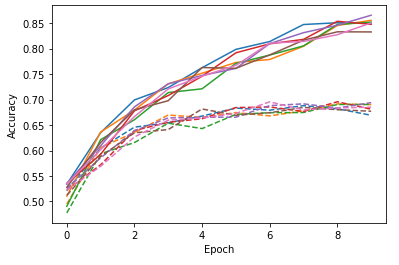
\includegraphics[width=0.5\textwidth]{code/A4d.png}
        \begin{minted}{python}
import torch
import torchvision
import torchvision.transforms as transforms
import numpy as np

device = torch.device('cuda:0' if torch.cuda.is_available() else 'cpu')
print(device)

transform = transforms.Compose(
    [transforms.ToTensor(),
     transforms.Normalize((0.5, 0.5, 0.5), (0.5, 0.5, 0.5))])

trainset = torchvision.datasets.CIFAR10(root='./data', train=True,
                                        download=True, transform=transform)
trainloader = torch.utils.data.DataLoader(trainset, batch_size=4,
                                          shuffle=True, num_workers=2)

testset = torchvision.datasets.CIFAR10(root='./data', train=False,
                                       download=True, transform=transform)
testloader = torch.utils.data.DataLoader(testset, batch_size=4,
                                         shuffle=False, num_workers=2)

classes = ('plane', 'car', 'bird', 'cat',
           'deer', 'dog', 'frog', 'horse', 'ship', 'truck')

import torch.nn as nn
import torch.nn.functional as F


class Net(nn.Module):
    def __init__(self, o1=6, k1=5, p=2, o2=16, k2=5, o3=120, o4=84):
        super(Net, self).__init__()
        self.conv1 = nn.Conv2d(3, o1, k1)
        self.pool = nn.MaxPool2d(p, p)
        self.conv2 = nn.Conv2d(o1, o2, k2)
        self.i3 = int(o2 * np.floor((np.floor((33-k1)/p)+1-k2)/p)**2)
        self.fc1 = nn.Linear(self.i3, o3)
        self.fc2 = nn.Linear(o3, o4)
        self.fc3 = nn.Linear(o4, 10)

    def forward(self, x):
        x = self.pool(F.relu(self.conv1(x)))
        x = self.pool(F.relu(self.conv2(x)))
        x = x.view(-1, self.i3)
        x = F.relu(self.fc1(x))
        x = F.relu(self.fc2(x))
        x = self.fc3(x)
        return x

import torch.optim as optim

criterion = nn.CrossEntropyLoss()

results = dict()

for j in range(20):

    o1 = np.random.randint(100,200)
    k1 = 5
    o2 = np.random.randint(100,200)
    k2 = 5
    p  = 3
    o3 = np.random.randint(60,200)
    o4 = np.random.randint(40,200)
    print(o1,k1,o2,k2,p,o3,o4)

    net = Net(o1=o1, o2=o2, o3=o3, o4=o4, k1=k1, k2=k2, p=p)
    net.to(device)

    optimizer = optim.SGD(net.parameters(), lr=0.001, momentum=0.9)

    losses = []
    train_acc = []
    val_acc = []
    for epoch in range(10):  # loop over the dataset multiple times

        running_loss = 0.0
        for i, data in enumerate(trainloader, 0):
            # get the inputs; data is a list of [inputs, labels]
            inputs, labels = data
            inputs, labels = inputs.to(device), labels.to(device)

            # zero the parameter gradients
            optimizer.zero_grad()

            # forward + backward + optimize
            outputs = net(inputs)
            loss = criterion(outputs, labels)
            loss.backward()
            optimizer.step()

            # print statistics
            running_loss += loss.item()
            if i % 2000 == 1999:    # print every 2000 mini-batches
                #print('[%d, %5d] loss: %.3f' %
                #      (epoch + 1, i + 1, running_loss / 2000))
                losses.append(running_loss / 2000)
                running_loss = 0.0

        # record the training accuracy
        correct = 0
        total = 0
        with torch.no_grad():
            for data in trainloader:
                images, labels = data
                images, labels = images.to(device), labels.to(device)
                outputs = net(images)
                _, predicted = torch.max(outputs.data, 1)
                total += labels.size(0)
                correct += (predicted == labels).sum().item()
        train_acc.append(correct/total)
        print('Train Acc', train_acc[-1])

        # record the validation accuracy
        correct = 0
        total = 0
        with torch.no_grad():
            for data in valloader:
                images, labels = data
                images, labels = images.to(device), labels.to(device)
                outputs = net(images)
                _, predicted = torch.max(outputs.data, 1)
                total += labels.size(0)
                correct += (predicted == labels).sum().item()
        val_acc.append(correct/total)

        results[j] = {'net': net,
                    'hp': {'o1': o1, 'o2': o2, 'o3': o3, 'o4': o4,
                           'k1': k1, 'k2': k2, 'p': p},
                    'losses': losses, 'train acc': train_acc, 'val acc': val_acc}
        print(j, f'{losses[-1]:.4f}')
        \end{minted}

        \newpage
        \item Before the perturbation, we get correctly classified images of a ship, bird, truck, and frog: \\
        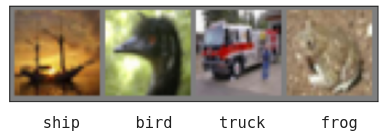
\includegraphics[width=0.4\textwidth]{code/A4e1.png} \\
        After the perturbation, the images look identical to the eye, but the network misclassifies all of them! \\
        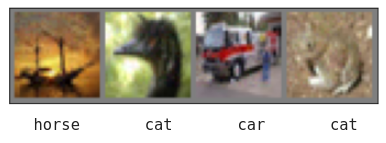
\includegraphics[width=0.4\textwidth]{code/A4e2.png} \\
        This is really peculiar.
        It suggests that the network isn't ``seeing'' the same features we are when we identify the images.
        It also suggests that the network is overfit -- it could totally fail on an almost identical set of images.
        However, it is not clear to me how ``artificial'' this new image set is.
        Perhaps, despite the fact that the images look the same to us, they are different in a way that is extremely unlikely to occur naturally.
        This seems plausible as we essentially added some noise in a \textit{perfectly} targeted way to degrade the classification.
        However, this could still be a problem if someone wanted to sneakily fool our algorithm.
        \begin{minted}{python}
# use network from before and create loss
net.eval()
lossFn = nn.CrossEntropyLoss()

# pick out 4 of the images
i = 0
for data, target in trainloader:
  data, target = data.to(device), target.to(device)
  i += 1
  if i == 4: break

# we want grads w.r.t. the images
data.requires_grad = True

# make predictions
output = net(data)
# calculate loss
loss = lossFn(output, target)

# take derivaties w.r.t. images
net.zero_grad()
loss.backward()

# get the sign of the data grad
sign_data_grad = data.grad.data.sign()

# perturb the images
epsilon = 0.05
perturbed_data = data + epsilon*sign_data_grad

# predict labels for perturbed images
perturbed_output = net(perturbed_data) 

import matplotlib.pyplot as plt
import numpy as np

# function to show an image
def imshow(img):
    img = img / 2 + 0.5     # unnormalize
    npimg = img.cpu().detach().numpy()
    plt.imshow(np.transpose(npimg, (1, 2, 0)))
    plt.show()

# show original images
imshow(torchvision.utils.make_grid(data))
# print original labels
print(' '.join('%9s' % classes[output.argmax(axis=1)[j]] for j in range(4)))

# show perturbed images
imshow(torchvision.utils.make_grid(perturbed_data))
# print perturbed labels
print(' '.join('%9s' % classes[perturbed_output.argmax(axis=1)[j]] for j in range(4)))
        \end{minted}
\end{enumerate}


\newpage

A.6

\begin{enumerate}
        \item
        \begin{minted}{python}
import torch
from torch import nn
import torch.nn.functional as F

class Encoder(nn.Module):
    
    def __init__(self, V, h, T):
        super(Encoder, self).__init__()
        self.Wx = nn.Linear(V, h)
        self.Wh = nn.Linear(h, h)
        self.Wmu = nn.Linear(h, T)
        self.Wsig = nn.Linear(h, T)
        
    def forward(self, x):
        h = F.ReLU(self.Wh(F.ReLU(self.Wx(x))))
        mu = self.Wmu(h)
        sigma = torch.exp(self.Wsig(h))
        z = torch.normal(mu, sigma)
        return z, mu, sigma
        \end{minted}

        \item
        \begin{minted}{python}
class Decoder(nn.Module):
    
    def __init__(self, V, T):
        super(Decoder, self).__init__()
        self.B = nn.Linear(T, V, bias=False)
        
    def forward(self, z):
        theta = F.softmax(z)
        eta = F.softmax(self.B(theta))
        return eta
        \end{minted}
        I also created an \texttt{AutoEncoder} that combines the Encoder and Decoder:
        \begin{minted}{python}
class AutoEncoder(nn.Module):
    
    def __init__(self, V, h, T):
        super(AutoEncoder, self).__init__()
        self.encoder = Encoder(V, h, T)
        self.decoder = Decoder(V, T)
    
    def forward(self, x):
        z, mu, sigma = self.encoder(x)
        eta = self.decoder(z)
        return eta, z, mu, sigma
        \end{minted}

        \newpage
        \item
        \begin{minted}{python}
def lossFn(x, eta, mu, sigma):
    logpxz = (x*torch.log(eta)).sum(axis=1)
    KLD = 1/2*(sigma**2 + mu**2 - 1 - torch.log(sigma**2)).sum(axis=1)
    return -(logpxz - KLD)
        \end{minted}

        \item I rewrote the loss function to be an instance of a class.
        This way, the function can remember what the current value of $\alpha$ is, and update it on every call to the loss function.
        You just need to initialize the loss function via \texttt{lossfn = LossFn()} at the start of your training loop.
        The loss function will then automatically update $\alpha$ on each training loop.
        \begin{minted}{python}
class LossFn():
    
    def __init__(self, linear_scaling=1000):
        self.linear_scaling = linear_scaling
        self.alpha = 0
        
    def __call__(self, x, eta, mu, sigma):
        # get the current alpha
        alpha = self.alpha
        # update alpha, and make sure it stays in the range (0,1)
        self.alpha = np.clip(self.alpha + 1/self.linear_scaling, 0, 1)
        # calculate and return loss
        logpxz = (x*torch.log(eta)).sum(axis=1)
        KLD = 1/2*(sigma**2 + mu**2 - 1 - torch.log(sigma**2)).sum(axis=1)
        return -(logpxz - alpha*KLD)
        \end{minted}

        \newpage
        \item \, \\
        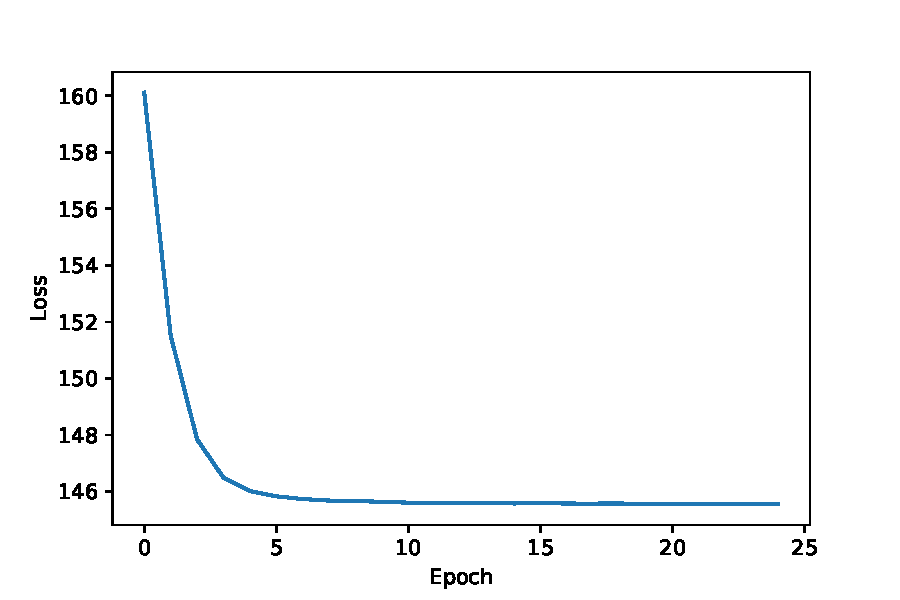
\includegraphics[width=0.7\textwidth]{code/A6e.pdf} \\
        \begin{minted}{python}
from helper_code import load_sparse, read_json, extract_topics, compute_npmi, generate_npmi_vals

# Compute data necessary to compute NPMI every epoch
reference_vocabulary = "reference/ref.vocab.json"
ref_counts = "reference/ref.npz"
ref_vocab = read_json(reference_vocabulary)
ref_vocab_index = dict(zip(ref_vocab, range(len(ref_vocab))))
# Loading reference count matrix.
ref_count_mat = load_sparse(ref_counts)
n_docs = ref_count_mat.shape[0]
# Computing word interaction matrix.
ref_doc_counts = (ref_count_mat > 0).astype(float)
ref_interaction = (ref_doc_counts).T.dot(ref_doc_counts)
ref_doc_sum = np.array(ref_doc_counts.sum(0).tolist()[0])
# Generating npmi matrices (which will be directly used to calculate nmpi).
(npmi_numerator,
 npmi_denominator) = generate_npmi_vals(ref_interaction, ref_doc_sum)

# load vocab and training matrix
vocabulary = read_json('vocabulary.json')
train = load_sparse('train.npz')

# Build a batch iterator
def batches(sparse, batch_size):
    i = 0
    while i + batch_size < sparse.shape[0]:
        yield torch.tensor(sparse[i:i+batch_size].toarray()).float()
        i += batch_size
    yield torch.tensor(sparse[i:].toarray()).float()

# create autoencoder
V = train.shape[1]
h = 81
T = 81
autoencoder = AutoEncoder(V, h, T)

# create the optimizer and loss function
optimizer = torch.optim.Adam(autoencoder.parameters(), lr=0.01)
lossfn = LossFn()

# arrays to save losses and npmis
losses = []
npmis = []

# Keep looping until npmi constant for P epochs
P = 5
Pcheck = np.arange(P, dtype=float)
epoch = 0
while not np.all(Pcheck == Pcheck[0]):
    
    # loop through batches
    batch_size = 64
    for i, batch in enumerate(batches(train, batch_size)):

        # evaluate autoencoder
        eta, z, mu, sigma = autoencoder(batch)

        # calculate loss
        loss = lossfn(batch, eta, mu, sigma).mean()
        
        # step optimizer
        optimizer.zero_grad()
        loss.backward()
        optimizer.step()
        
        # print loss every 400 iterations
        if i % 400 == 0: print(f'{loss.item():.3f}')
         
    # save loss at end of epoch
    losses.append(loss.item())
    
    # calculate and save npmi
    B = autoencoder.decoder.B.weight
    topics = extract_topics(B, list(vocab.keys()))
    npmi = compute_npmi(npmi_numerator, npmi_denominator, n_docs, ref_vocab_index, topics)
    npmis.append(npmi)
    Pcheck[epoch % P] = npmi
    print(f'NPMI = {npmi}')
    
    # advance epoch count!
    epoch += 1
        \end{minted}
\end{enumerate}




\newpage

B.1

\begin{enumerate}
        \item The test error is 1.064.
        Here is the code:
        \begin{minted}{python}
import numpy as np
import matplotlib.pyplot as plt
import csv

data = []
with open("u.data") as csvfile:
    spamreader = csv.reader(csvfile, delimiter="\t")
    for row in spamreader:
        data.append([int(row[0])-1, int(row[1])-1, int(row[2])])
data = np.array(data)

num_observations = len(data) # num_observations = 100,000
num_users = max(data[:,0])+1 # num_users = 943, indexed 0,...,942
num_items = max(data[:,1])+1 # num_items = 1682 indexed 0,...,1681

np.random.seed(1)
num_train = int(0.8*num_observations)
perm = np.random.permutation(data.shape[0])
train = data[perm[0:num_train],:]
test = data[perm[num_train::],:]

# get the list of every movie
movies = list(set(data[:,1]))

# dictionaries to calculate mean score
scores = {m: 0 for m in movies}
count = {m: 0 for m in movies}

# sum up totals
for user, movie, score in train:
    scores[movie] += score
    count[movie] += 1

# calculate mean scores
for movie in scores:
    N = max(count[movie], 1)
    scores[movie] /= N
    
# calculate test error
err = np.mean((test[:,2] - np.vectorize(scores.get)(test[:,1]))**2)
print(f'Test Error = {err:.3f}')
        \end{minted}

        \newpage
        \item \, \\
        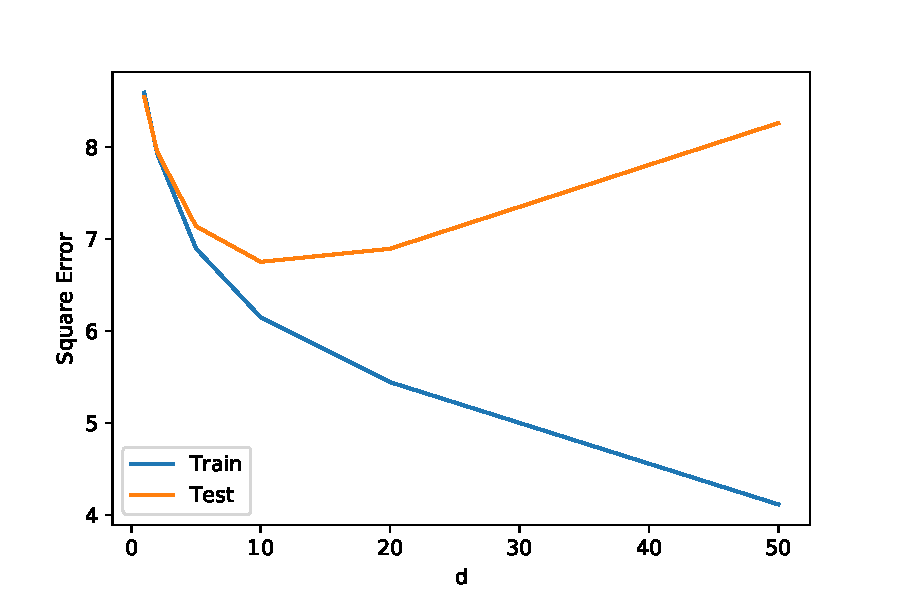
\includegraphics[width=0.7\textwidth]{code/B1b.pdf}
        \begin{minted}{python}
import numpy as np
import matplotlib.pyplot as plt
import csv

data = []
with open("u.data") as csvfile:
    spamreader = csv.reader(csvfile, delimiter="\t")
    for row in spamreader:
        data.append([int(row[0])-1, int(row[1])-1, int(row[2])])
data = np.array(data)

num_observations = len(data) # num_observations = 100,000
num_users = max(data[:,0])+1 # num_users = 943, indexed 0,...,942
num_items = max(data[:,1])+1 # num_items = 1682 indexed 0,...,1681

np.random.seed(1)
num_train = int(0.8*num_observations)
perm = np.random.permutation(data.shape[0])
train = data[perm[0:num_train],:]
test = data[perm[num_train::],:]

from scipy.sparse.linalg import svds

Rtrain = np.zeros((num_items, num_users))
Rtrain[train[:,1], train[:,0]] = train[:,2]

Rtest = np.zeros((num_items, num_users))
Rtest[test[:,1], test[:,0]] = test[:,2]

train_err = []
test_err = []
ds = [1,2,5,10,20,50]
for d in ds:
    U, S, VH = svds(Rtrain, k=d)
    Rhat = U @ (S[..., None] * VH)
    Rhat = Rhat.flatten()
    
    Rtrain_ = Rtrain.flatten()
    idx = np.where(Rtrain_ != 0)
    train_err.append(np.mean((Rtrain_[idx] - Rhat[idx])**2))

    Rtest_ = Rtest.flatten()
    idx = np.where(Rtest_ != 0)
    test_err.append(np.mean((Rtest_[idx] - Rhat[idx])**2))

plt.plot(ds, train_err, label='Train')
plt.plot(ds, test_err, label='Test')
plt.legend()
plt.xlabel('d')
plt.ylabel("Error") 
        \end{minted}

        \newpage
        \item We want to minimize the objective
        \begin{align*}
                \min_X \norm{M \circ (AX - Y)}^2 + \lambda \norm{X}^2,
        \end{align*}
        where $M$ is a mask with 0's for missing values in A and Y, and $\circ$ is the Hadamard product.
        We can rewrite the objective in terms of the trace:
        \begin{align*}
                \mathrm{Tr}[(X^T A^T (M \circ AX))] - 2 \mathrm{Tr}[X^T A^T (M \circ Y)] + \mathrm{Tr}[Y^T(M \circ Y)] + \lambda \mathrm{Tr}[X^T X].
        \end{align*}
        Now using formulae from the Matrix Cookbook to take the derivative with respect to $X$, setting equal to zero, and dividing by 2:
        \begin{align*}
                A^T (M \circ AX) - A^T (M \circ Y) + \lambda X = 0.
        \end{align*}
        Now evaluating the first term:
        \begin{align*}
                [A^T (M \circ AX)]_{kl}
                &= \sum_i A_{il} M_{ik} \sum_j A_{ij} X_{jk} \\
                &= \sum_j \left( \sum_i A_{il} M_{ik} A_{ij} \right) X_{jk},
        \end{align*}
        where the term in parentheses is a tensor I will name $T$.
        Finally, we can write our solution as 
        \begin{align*}
                (A^T T A + \lambda I) X = A^T (M \circ Y).
        \end{align*}
        Now by appropriately constructing $T$ and evaluating everything except for $X$, we can solve for $X$ using \texttt{np.linalg.solve}.
        Using this solution, we can alternate back and forth, solving for $U$ and $V$.
        I initialize the $v$ and $u$ using the SVD decompositions from part b and found that $\lambda = 10$ worked best. \\
        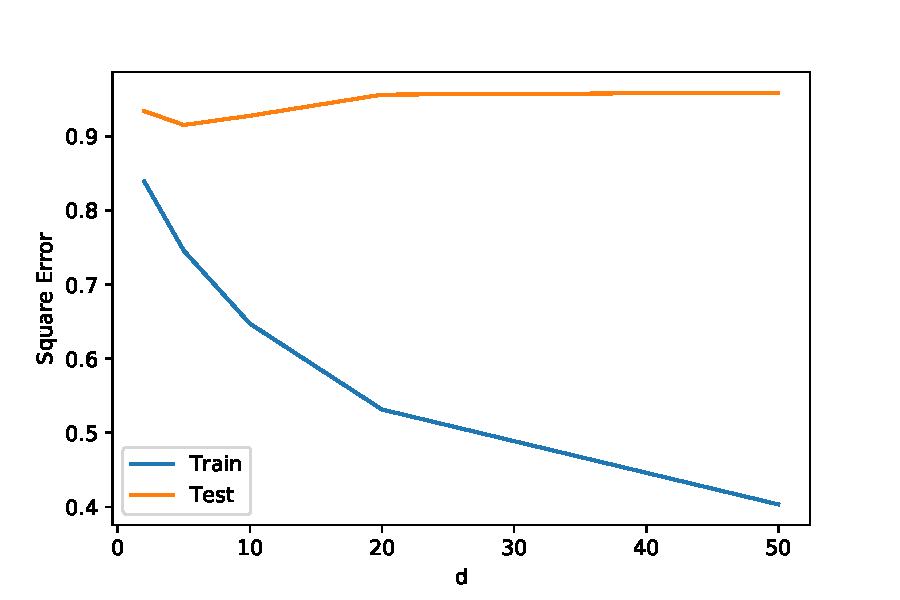
\includegraphics[width=0.7\textwidth]{code/B1c.pdf} \\
        You can see that $d=5$ generalizes the best.
        Here is the code:
        \begin{minted}{python}
import numpy as np
import matplotlib.pyplot as plt
import csv

data = []
with open("u.data") as csvfile:
    spamreader = csv.reader(csvfile, delimiter="\t")
    for row in spamreader:
        data.append([int(row[0])-1, int(row[1])-1, int(row[2])])
data = np.array(data)

num_observations = len(data) # num_observations = 100,000
num_users = max(data[:,0])+1 # num_users = 943, indexed 0,...,942
num_items = max(data[:,1])+1 # num_items = 1682 indexed 0,...,1681

np.random.seed(1)
num_train = int(0.8*num_observations)
perm = np.random.permutation(data.shape[0])
train = data[perm[0:num_train],:]
test = data[perm[num_train::],:]

Rtrain = np.zeros((num_users, num_items))
Rtrain[train[:,0], train[:,1]] = train[:,2]

Rtest = np.zeros((num_users, num_items))
Rtest[test[:,0], test[:,1]] = test[:,2]

from scipy.sparse.linalg import svds

def lstsq_missing_vals(A, B, M, lam=10):
    rhs = (A.T @ (M * B)).T[:,:,None]
    T = A.T[None,:,:] @ (M.T[:,:,None] * A[None,:,:])
    Id = lam * np.identity(T.shape[1])[None,...]
    return np.linalg.solve(T + Id, rhs).squeeze().T

    train_err = []
test_err = []
ds = [2,5,10,20,50]
for d in ds:
    print(d)
    
    U, S, VH = svds(Rtrain, k=d)
    U_ = 0 * U
    VH = S[..., None] * VH
    VH_ = 0 * VH

    M = Rtrain.clip(0,1)

    while not np.allclose(U, U_) or not np.allclose(VH, VH_):
        U_, VH_ = U, VH
        VH = lstsq_missing_vals(U, Rtrain, M)
        U = lstsq_missing_vals(VH.T, Rtrain.T, M.T).T
        
    Rhat = U @ VH
    Rhat = Rhat.flatten()

    Rtrain_ = Rtrain.flatten()
    idx = np.where(Rtrain_ != 0)
    train_err.append(np.mean((Rtrain_[idx] - Rhat[idx])**2))

    Rtest_ = Rtest.flatten()
    idx = np.where(Rtest_ != 0)
    test_err.append(np.mean((Rtest_[idx] - Rhat[idx])**2))    
        \end{minted}
\end{enumerate}

\newpage

A.7

\begin{enumerate}
    \item We can use a simple counter example to show this space is not convex.
    Consider the matrices $A = \begin{pmatrix} 1 & 0 \\ 0 & 0 \end{pmatrix}$ and $B = \begin{pmatrix} 0 & 0 \\ 0 & 1 \end{pmatrix}$, both of which are rank 1.
    We say a set $S$ is convex if $\lambda A + (1-\lambda) B \in S$ for all $A,B \in C$ and $\lambda \in [0,1]$.
    Well 
    \begin{align*}
        \lambda A + (1-\lambda) B = 
        \begin{pmatrix}
            \lambda & 0 \\ 0 & 1-\lambda
        \end{pmatrix}
    \end{align*}
    is rank 2 for $\lambda \in (0,1)$, so this set is obviously non-convex.

    \item 
    \begin{enumerate}
        \item The closest point in the span of $\{w_j\}$ is the projection of the vector onto the span.
        This is equal to
        \begin{align*}
            v = \sum_j X_{(i)}^{*T} w_j.
        \end{align*}

        \item Since these vectors are orthonormal, there exists a basis in which $\Pi = \mathbf{I}_{k \times k} \oplus \mathbf{0}_{(n-k) \times (n-k)}$.
        Then we can trivially take the SVD of each block separately.
        This makes it obvious that $\Pi$ has $k$ singular values equal to 1 and $n-k$ singular values equal to 0.

        \item Again, we can consider $\Pi$ in the basis where $\Pi = \mathbf{I}_{k \times k} \oplus \mathbf{0}_{(n-k) \times (n-k)}$.
        In this basis, it is obvious:
        \begin{align*}
            \Pi^2 
            &= (\mathbf{I}_{k \times k} \oplus \mathbf{0}_{(n-k) \times (n-k)})
            (\mathbf{I}_{k \times k} \oplus \mathbf{0}_{(n-k) \times (n-k)}) \\
            &= \mathbf{I}_{k \times k}^2 \oplus \mathbf{0}_{(n-k) \times (n-k)}^2 \\
            &= \mathbf{I}_{k \times k} \oplus \mathbf{0}_{(n-k) \times (n-k)} = \Pi.
        \end{align*}
        We can also see this by letting $P$ be the change of basis matrix such that 
        \begin{align*}
            \Pi = 
            P^{-1} (\mathbf{I}_{k \times k} \oplus \mathbf{0}_{(n-k) \times (n-k)}) P.
        \end{align*}
        Then, 
        \begin{align*}
            \Pi^2 &= 
            P^{-1} (\mathbf{I}_{k \times k} \oplus \mathbf{0}_{(n-k) \times (n-k)}) P
            P^{-1} (\mathbf{I}_{k \times k} \oplus \mathbf{0}_{(n-k) \times (n-k)}) P \\
            &= 
            P^{-1} (\mathbf{I}_{k \times k} \oplus \mathbf{0}_{(n-k) \times (n-k)})^2 P \\
            &= P^{-1} (\mathbf{I}_{k \times k}^2 \oplus \mathbf{0}_{(n-k) \times (n-k)}^2) P \\
            &= P^{-1} (\mathbf{I}_{k \times k} \oplus \mathbf{0}_{(n-k) \times (n-k)}) P
            = \Pi
        \end{align*}

        \item Since these new vectors are orthonormal, there exists a basis in which
        \begin{align*}
            \sum_{i=k+1}^n w_i w_i^T 
            = \mathbf{0}_{k \times k} \oplus \mathbf{I}_{(n-k) \times (n-k)}.
        \end{align*}
        Thus, we can write
        \begin{align*}
            \sum_{i=1}^n w_i w_i^T 
            &= \sum_{i=1}^k w_i w_i^T + \sum_{i=k+1}^n w_i w_i^T \\
            &= \mathbf{I}_{k \times k} \oplus \mathbf{0}_{(n-k) \times (n-k)}
            + \mathbf{0}_{k \times k} \oplus \mathbf{I}_{(n-k) \times (n-k)} \\
            &= (\mathbf{I}_{k \times k} + \mathbf{0}_{k \times k})
            \oplus (\mathbf{0}_{(n-k) \times (n-k)} + \mathbf{I}_{(n-k) \times (n-k)}) \\
            &= \mathbf{I}_{k \times k} \oplus \mathbf{I}_{(n-k) \times (n-k)} 
            = \mathbf{I}_{n \times n}
        \end{align*}
    \end{enumerate}

    \item
    \begin{enumerate}
        \item
        \begin{align*}
            \norm{\hat{X} - X^*}_F^2 
            &= \norm{(\Pi - I)X^*}_F^2
            = \norm{\left(\sum_{i=1}^k w_i w_i^T - \sum_{i=1}^n w_i w_i^T \right)X^*}_F^2 \\
            &= \norm{\left(\sum_{i=k+1}^n w_i w_i^T\right)X^*}_F^2
            = \norm{\Pi^\perp X^*}_F^2
        \end{align*}

        \item
        \begin{align*}
            \norm{\Pi^\perp X^*}_F^2 
            &= \mathrm{Tr}((\Pi^\perp X^*) (\Pi^\perp X^*)^T) & \text{Definition of Frobenius Norm}\\
            &= \mathrm{Tr}(\Pi^\perp X^* X^{*T} \Pi^\perp) & \text{Symmetry of } \Pi / \Pi^\perp \\
            &= \mathrm{Tr}(X^* X^{*T} \Pi^\perp \Pi^\perp) & \text{Cyclic property of trace} \\
            &= \mathrm{Tr}(X^* X^{*T} \Pi^\perp) & \text{Idempotency of } \Pi / \Pi^\perp
        \end{align*}

        \item 
        \begin{align*}    
            X^* X^{*T} \Pi^\perp
            &= \left( \sum_{i=1}^n \sigma_i u_i v_i^T \right)
            \left( \sum_{j=1}^n \sigma_j u_j v_j^T \right)^T
            \left( \sum_{l=k+1}^n w_l w_l^T \right) \\
            &= \sum_{\substack{i=1 \\ j=1 \\ l=k+1}}^n 
            \sigma_i \sigma_j u_i v_i^T v_j u_j^T w_l w_l^T
            = \sum_{\substack{i=1 \\ j=1 \\ l=k+1}}^n
            \sigma_i \sigma_j u_i \delta_{ij} u_j^T w_l w_l^T \\
            &= \sum_{\substack{i=1 \\ l=k+1}}^n 
            \sigma_i^2 u_i u_i^T w_l w_l^T 
            = \sum_{i=1}^n \sigma_i^2 \sum_{l=k+1}^n w_l w_l^T
        \end{align*}
        Then taking the trace:
        \begin{align*}
            \mathrm{Tr}(X^* X^{*T} \Pi^\perp)
            = \sum_{i=1}^n \sigma_i^2 (n-k)
            \geq \sum_{i=k+1}^n \sigma_i^2
        \end{align*}
    \end{enumerate}

    \begin{enumerate}
        \item The minimum is then clearly the equality of the above relation, which via (a) and (b) I showed was equivalent to $\norm{X-X^*}_F^2$.
        \item The best rank-$k$ approximation is formed by taking the SVD, ordering the singular values and corresponding vectors in ascending order, then using
        \begin{align*}
            \hat{X} = \sum_{i=1}^k \sigma_i u_i v_i^T
        \end{align*}
    \end{enumerate}
\end{enumerate}


\end{document}